\documentclass[portrait,a1,posterdraft]{a0poster}\usepackage[]{graphicx}\usepackage[]{xcolor}
% maxwidth is the original width if it is less than linewidth
% otherwise use linewidth (to make sure the graphics do not exceed the margin)
\makeatletter
\def\maxwidth{ %
  \ifdim\Gin@nat@width>\linewidth
    \linewidth
  \else
    \Gin@nat@width
  \fi
}
\makeatother

\definecolor{fgcolor}{rgb}{0.345, 0.345, 0.345}
\newcommand{\hlnum}[1]{\textcolor[rgb]{0.686,0.059,0.569}{#1}}%
\newcommand{\hlstr}[1]{\textcolor[rgb]{0.192,0.494,0.8}{#1}}%
\newcommand{\hlcom}[1]{\textcolor[rgb]{0.678,0.584,0.686}{\textit{#1}}}%
\newcommand{\hlopt}[1]{\textcolor[rgb]{0,0,0}{#1}}%
\newcommand{\hlstd}[1]{\textcolor[rgb]{0.345,0.345,0.345}{#1}}%
\newcommand{\hlkwa}[1]{\textcolor[rgb]{0.161,0.373,0.58}{\textbf{#1}}}%
\newcommand{\hlkwb}[1]{\textcolor[rgb]{0.69,0.353,0.396}{#1}}%
\newcommand{\hlkwc}[1]{\textcolor[rgb]{0.333,0.667,0.333}{#1}}%
\newcommand{\hlkwd}[1]{\textcolor[rgb]{0.737,0.353,0.396}{\textbf{#1}}}%
\let\hlipl\hlkwb

\usepackage{framed}
\makeatletter
\newenvironment{kframe}{%
 \def\at@end@of@kframe{}%
 \ifinner\ifhmode%
  \def\at@end@of@kframe{\end{minipage}}%
  \begin{minipage}{\columnwidth}%
 \fi\fi%
 \def\FrameCommand##1{\hskip\@totalleftmargin \hskip-\fboxsep
 \colorbox{shadecolor}{##1}\hskip-\fboxsep
     % There is no \\@totalrightmargin, so:
     \hskip-\linewidth \hskip-\@totalleftmargin \hskip\columnwidth}%
 \MakeFramed {\advance\hsize-\width
   \@totalleftmargin\z@ \linewidth\hsize
   \@setminipage}}%
 {\par\unskip\endMakeFramed%
 \at@end@of@kframe}
\makeatother

\definecolor{shadecolor}{rgb}{.97, .97, .97}
\definecolor{messagecolor}{rgb}{0, 0, 0}
\definecolor{warningcolor}{rgb}{1, 0, 1}
\definecolor{errorcolor}{rgb}{1, 0, 0}
\newenvironment{knitrout}{}{} % an empty environment to be redefined in TeX

\usepackage{alltt}

\usepackage{epsf,pstricks}
\usepackage[utf8]{inputenc}

\usepackage{amsmath}
\usepackage[T1]{fontenc}

%\usepackage{hyperref}
\usepackage{geometry}
\geometry{verbose,tmargin=1.0cm,bmargin=1.5cm,lmargin=1.5cm,rmargin=1.5cm}
\setcounter{secnumdepth}{2}
\setcounter{tocdepth}{2}
\usepackage{url}
\usepackage[unicode=true,pdfusetitle,
 bookmarks=true,bookmarksnumbered=true,bookmarksopen=true,bookmarksopenlevel=2,
 breaklinks=ning,pdfborder={0 0 1},backref=ning,colorlinks=ning]
 {hyperref}
\hypersetup{pdfstartview={XYZ null null 1}}
\usepackage{nopageno}
\usepackage{authblk}
\usepackage{tikz}
\usetikzlibrary{shapes,arrows,snakes}
\usepackage{amsmath,amssymb}
\usetikzlibrary{positioning}




% Define block styles


\title{Modelling of degree distribution }
\author{Thomas Boughen}
\date{}

\usepackage{framed}
\usepackage{xcolor,eso-pic}
\usepackage{svg}

\definecolor{header}{HTML}{8fbdbd}
\pagecolor{header!80}
\AddToShipoutPictureBG{
  \AtPageLowerLeft{%
    \color{header!20}%
    \rule{\pdfpagewidth}{0.885\pdfpageheight}%
  }
}
\IfFileExists{upquote.sty}{\usepackage{upquote}}{}
\begin{document}

  \pagestyle{empty}
  \fontfamily{phv}\selectfont



  
  \maketitle
  
  
  
  
  
  
  \tikzstyle{decision} = [diamond, draw, fill=blue!20, text width=4.5em, text badly centered, node distance=3cm, inner sep=0pt]
  \tikzstyle{block} = [rectangle, draw, fill=blue!20, text width=5em, text centered, rounded corners, minimum height=4em]
  \tikzstyle{greenbox} = [rectangle, draw=blue, fill=green!20, text width=5em, text centered, rounded corners, inner sep=10pt, inner ysep=12pt, very thick]
  \tikzstyle{line} = [draw, -latex']
  \tikzstyle{cloud} = [draw, ellipse, node distance=4cm, minimum height=2em, text width=5em]
  \tikzstyle{mybox} = [draw=blue, fill=green!20, very thick, rectangle, rounded corners, inner sep=10pt, inner ysep=20pt]
  \tikzstyle{myboxwhite} = [rectangle, rounded corners, inner sep=10pt, inner ysep=0pt]
  
  \tikzstyle{myboxblue} = [rectangle, fill=header!10, rounded corners, inner sep=10pt, inner ysep=20pt]
  
  \tikzstyle{myboxgreen} = [rectangle, fill=green!10, rounded corners, inner sep=10pt, inner ysep=20pt]
  \tikzstyle{fancytitle} = [fill=white, text=black, ellipse, draw=blue]
  
  
  
  
  \small
  
  \begin{tikzpicture}[]

\node [myboxblue,anchor=north west](abstract) at (0cm,0cm) {%
    \begin{minipage}{21cm}
              {\bf Abstract} Lorem ipsum dolor sit amet, consectetur adipiscing elit. Suspendisse aliquam ipsum id consequat euismod. In auctor faucibus mi, vitae blandit nunc vestibulum eget. Fusce eu venenatis dolor, a blandit metus. Aliquam congue congue molestie. Donec euismod bibendum felis a interdum. Vestibulum et euismod sapien, sed accumsan augue. Fusce vulputate arcu et dolor condimentum, a condimentum elit blandit. Nam in maximus lorem. Ut neque felis, hendrerit at orci non, sodales eleifend augue.

Duis convallis lacinia justo. Suspendisse imperdiet fermentum finibus. Praesent semper dignissim felis, eu lobortis ex pharetra eu. Pellentesque nec bibendum augue. Cras vulputate viverra finibus. Praesent facilisis quam vel nisi convallis congue. Nunc ullamcorper tristique sagittis.

    \end{minipage}
};

\node [myboxblue,right of = abstract,xshift=21cm,anchor=north west](Power Law) at (0,0) {%
    \begin{minipage}{21cm}
              {\bf Power Law Model} \\
              \\
              We first consider the model that is often assumed for degree distributions in order to show how well (or poorly) it fits the data. This model, describes the data using the probability mass function:
              $$
              f(x) = \zeta(\alpha+1)^{-1} x^{-(\alpha+1)}\qquad x=1,2,\ldots \quad \text{and }  \alpha>0
              $$
              It is possible to fit this model using maximum likelihood, however since we will be using a Bayesian methodology for the other models, it is prudent we do so here as well. First we need the likelihood for a set of data $\boldsymbol{x} = (x_1,x_2,\ldots, x_N)^T$
              $$
              L(\boldsymbol{x}) = \zeta(\alpha+1)^{-N}\prod_{i=1}^N x_i^{-(\alpha+1)}
              $$
              Then we need to decide on a prior for $\alpha$, since it is restricted to the positive real line, we will use $\alpha \sim Ga(1,\lambda_\alpha)$.With this, we can now calculate the posterior distribution :
              $$
              \pi(\alpha|\boldsymbol{x}) = \zeta(\alpha+1)^{-N}\prod_{i=1}^N x_i^{-(\alpha+1)}\lambda_\alpha e^{-\alpha\lambda_\alpha}
              $$
              
              \vspace{7.5cm}
    \end{minipage}
};

\node [myboxblue,right of = Power Law,xshift=22cm,anchor=north west](Aside) at (21,0) {%
    \begin{minipage}{11cm}
              {\bf What is a network?}\\
              \\
              A network is a collection of nodes with edges between them, these edges can be directed or undirected. The nodes and edges can represent a vast number of things, but representing them in this way allows us to analyse the structure of what is being represented more easily. The degree of a node is the number of edges that are connected to it, with the in-degree and out-degree being the number going in and out respectively. An example is below:
\begin{knitrout}
\definecolor{shadecolor}{rgb}{0.969, 0.969, 0.969}\color{fgcolor}
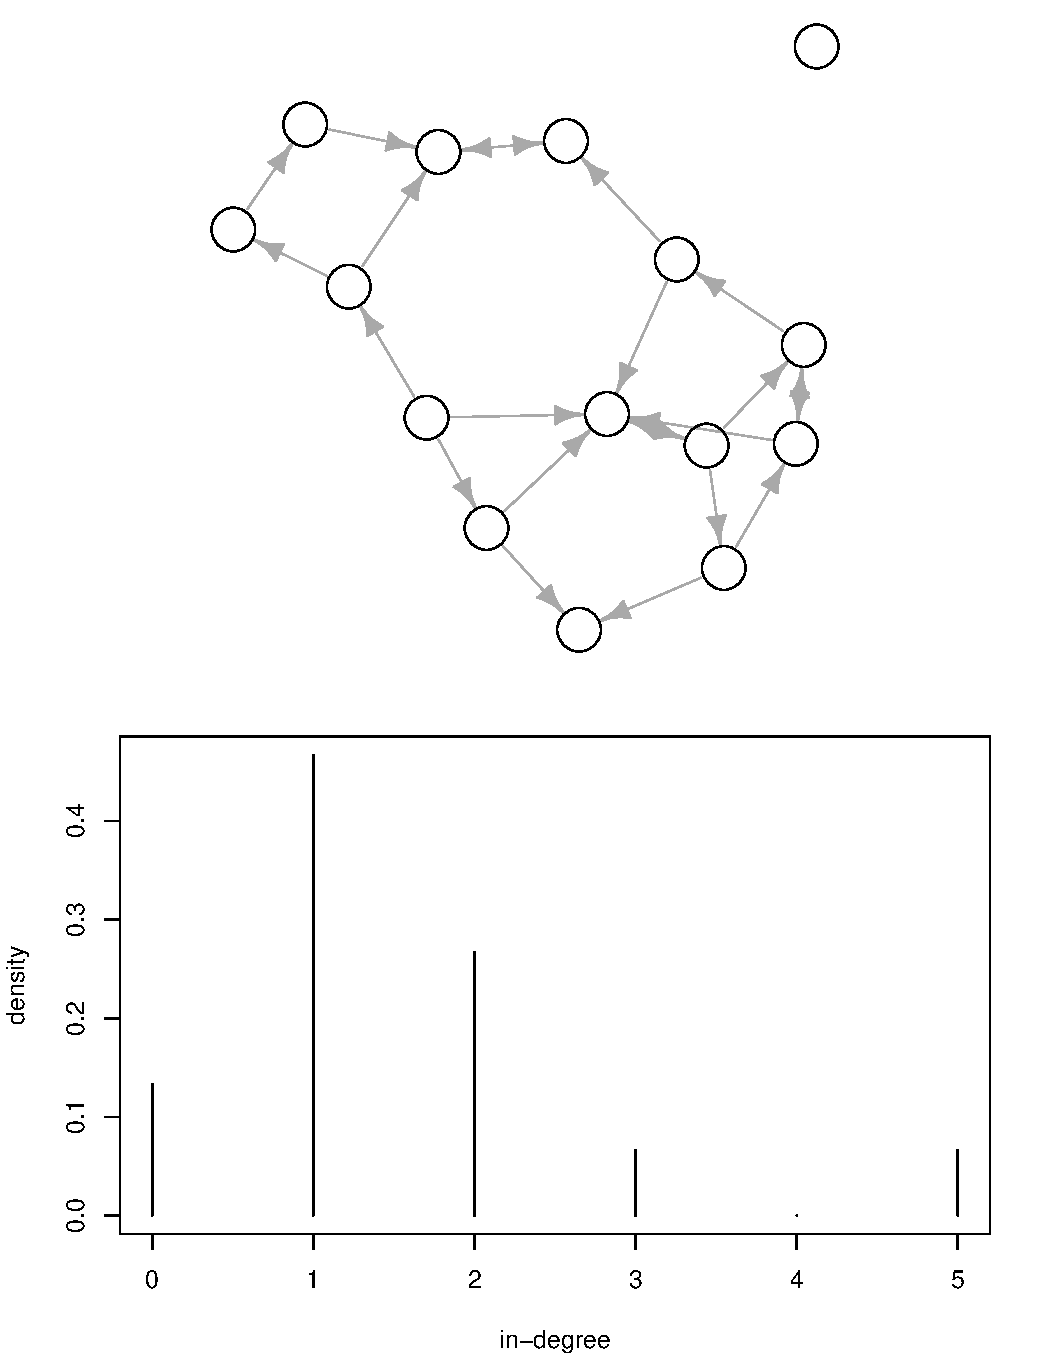
\includegraphics[width=\maxwidth]{figure/unnamed-chunk-1-1} 
\end{knitrout}
    \end{minipage}
};

\node [myboxblue,below of = abstract,yshift=0cm,anchor=north west](Data) at (0,-15) {%
    \begin{minipage}{21cm}
              {\bf Data}\\
              \\
              Here we will be looking at the degree distribution of one specific network, the network of dependencies of packages from the Comprehensive R Archive Network (CRAN). This data forms a network in that, each of the packages has a node and there exists a directed edge between node A and node B if package B depends on package A. We will only be considering the in-degree of nodes of this network as it is more analagous to other real world networks e.g. social media followers.\\
              
              However this data has a significant number of zeroes that are mostly uninteresting, but will skew the data enough to effect the fit of the models. So, we will be ignoring them from now on, and if we wanted to model them we would model them separately.
    \end{minipage}
};

\node [myboxblue,below of = Data,yshift=0cm,anchor=north west](PowerPower) at (0,-30) {%
    \begin{minipage}{27cm}
              {\bf Power Law Mixture} \\
              \\
              Based on [ref plot] it is seems natural to consider using a mixture of two power laws to
              model the data. This model assigns the following probability mass function to the data:
              $$
              f(x) = \begin{cases}
              (1-\phi)[\zeta(\alpha+1) - \zeta_v(\alpha+1)]^{-1}x^{-(\alpha+1)}&, x = 1,2,\ldots,v\\
              \phi \zeta_v(\beta+1)^{-1}x^{-(\beta+1)}&,x=v+1,v+2,\ldots
              \end{cases}
              $$
              where $\alpha,\beta \in \mathbb{R}^+, \phi \in (0,1), v = \lceil u \rceil$ or $\lfloor u \rfloor$, $u\in \mathbb{R}^+$ and $\zeta_v(s) =                 \sum_{k=v+1}^\infty  k^{-s}.$ \\
              \\
              We decide to use the maximum likelihood estimator of $\phi$, $\hat \phi  = \frac{N-n}{N}$, and decide to use $u$ as an integer between 0 and $N-1$ since in this network no node can have in-degree more than $N-1$.\\ 
              \\
              The priors for the unknown parameters are below:
              \begin{align*}
              &\alpha \sim Ga(1,\lambda_\alpha) &\beta \sim Ga(1,\lambda_\beta)& &u\sim U(0,N-1) 
              \end{align*}
              \\
              We can now obtain the posterior distribution:
              $$
              \pi(\alpha,\beta,u|\boldsymbol{x}) = \frac{\lambda_\alpha\lambda_\beta n^n (N-n)^{N-n}}{N^{N+1}}\zeta_u(\beta+1)^{n-N}[\zeta(\alpha+1) - \zeta_v(\alpha+1)]^{-n} \prod_{i=1}^N x_i^{-(\gamma_i +1)}
              $$
              where $\gamma_i = \alpha$ if $x_i\le u$ or $\gamma_i = \beta$ if $x_i > u$, and $n = \text{number of }x_i \le u$.
              \vspace{4.13cm}
              
    \end{minipage}
};


\node [myboxblue,right of = PowerPower,yshift=-1cm,xshift=0cm,anchor=north west](PowerIgpd) at (27,-30) {%
    \begin{minipage}{27cm}
              {\bf Power Law-Integrated Generalised Pareto Mixture Model} 
              \\
              \\
              We naturally look to extreme value theory, specifically using a threshold model. The distribution typically used to describe the distribution of excesses of a threshold is the Generalised Pareto Distribution, but this is only defined for continuous data so we look to using the Integrated Generalised Pareto Distrubtion [CITE] with threshold $v\in \mathbb{Z}^+$, which has probability mass function:
              $$
              g(y) =\left(1+\frac{\xi(y-v-1)}{\sigma_0 + \xi\ v}\right)_+^{-1/\xi} -\left(1+\frac{\xi(y-v)}{\sigma_0 + \xi\ v}\right)_+^{-1/\xi},\qquad y=v+1,v+2,\ldots
              $$
              where $\xi \in \mathbb{R},\sigma_0 \in \mathbb{R}^+$.\\
              \\
            Our mixture distribution then has probability mass function:
            
            $$
            f(x) = \begin{cases}
            (1-\phi)[\zeta(\alpha+1) - \zeta_v(\alpha+1)]^{-1} x^{-(\alpha+1)}&, x=1,2,\ldots,v\\
            \phi g(x)&,x=v+1,v+2,\ldots
            \end{cases}
            $$
            where $\alpha\in \mathbb{R}^+, \phi\in (0,1)$ and $\zeta_v(s) = \sum_{k=v+1}^\infty k^{-s}.$\\
            \\
            We can set $v = \lfloor u \rfloor \text{ or } \lceil u \rceil$, $u\in \mathbb{R}^+$, here we will set $u\in \mathbb{Z}^+$ and $v=u$\\
            \\
            We decide on the priors below for the parameters and use the MLE $ (\hat \phi=\frac{N-n}{N})$:
            $$
            \alpha \sim Ga(1,\lambda_\alpha),\, \sigma_0\sim Ga(1,\lambda_\sigma),\,\xi \sim N(0,\,\lambda_\xi^2),\,u\sim U(0,N-1)
            $$
            and obtain the posterior:
            $$
            \pi(\alpha,\sigma_0, \xi | \boldsymbol{x}) = \frac{\lambda_\alpha \lambda_\sigma n^n (N-n)^{N-n}e^{-(\alpha\lambda_\alpha + \sigma_0\lambda_\sigma + \frac{\xi^2}{2\lambda_\sigma^2})}}{N^{N+1}[\zeta(\alpha+1) - \zeta_v(\alpha+1)]^n} \prod_{i:x_i \le v}x_i ^{-(\alpha+1)}\prod_{i:x_i>v}g(x_i)
            $$
          
           
    \end{minipage}
};




\node [myboxblue,below of = PowerPower,yshift=0cm,anchor=north west](Plots) at (0,-59) {%
    \begin{minipage}{43cm}
              {\bf Plots} Lorem ipsum dolor sit amet, consectetur adipiscing elit. Suspendisse aliquam ipsum id consequat euismod. In auctor faucibus mi, vitae blandit nunc vestibulum eget. Fusce eu venenatis dolor, a blandit metus. Aliquam congue congue molestie. Donec euismod bibendum felis a interdum. Vestibulum et euismod sapien, sed accumsan augue. Fusce vulputate arcu et dolor condimentum, a condimentum elit blandit. Nam in maximus lorem. Ut neque felis, hendrerit at orci non, sodales eleifend augue.

Duis convallis lacinia justo. Suspendisse imperdiet fermentum finibus. Praesent semper dignissim felis, eu lobortis ex pharetra eu. Pellentesque nec bibendum augue. Cras vulputate viverra finibus. Praesent facilisis quam vel nisi convallis congue.
Duis convallis lacinia justo. Suspendisse imperdiet fermentum finibus. Praesent semper dignissim felis, eu lobortis ex pharetra eu. Pellentesque nec bibendum augue. Cras vulputate viverra finibus. Praesent facilisis quam vel nisi convallis congue.
Duis convallis lacinia justo. Suspendisse imperdiet fermentum finibus. Praesent semper dignissim felis, eu lobortis ex pharetra eu. Pellentesque nec bibendum augue. Cras vulputate viverra finibus. Praesent facilisis quam vel nisi convallis congue.Duis convallis lacinia justo. Suspendisse imperdiet fermentum finibus. Praesent semper dignissim felis, eu lobortis ex pharetra eu. Pellentesque nec bibendum augue. Cras vulputate viverra finibus. Praesent facilisis quam vel nisi convallis congue.
    \end{minipage}
};


\node [myboxblue,right of = Plots,yshift=0cm,anchor=north west](future) at (43,-60) {%
    \begin{minipage}{11cm}
              {\bf Future} Lorem ipsum dolor sit amet, consectetur adipiscing elit. Suspendisse aliquam ipsum id consequat euismod. Lorem ipsum dolor sit amet, consectetur adipiscing elit. Suspendisse aliquam ipsum id consequat euismod. 
             Lorem ipsum dolor sit amet, consectetur adipiscing elit. Suspendisse aliquam ipsum id consequat euismod. 
             
             
             
              
    \end{minipage}
};











\end{tikzpicture}


\end{document}
